\subsection{Projeto de Hardware}

O projeto geral de hardware está descrito na Figura \ref{fig-projetoGeralHardware}. O mesmo foi feito levando em consideração os requisitos funcionais citados no relatório do Ponto de Controle 1 \cite{relPC1}.  Os principais componentes do diagrama abaixo serão tratados individualmente nas secções a seguir.

\begin{figure}[htbp]
	\centering
		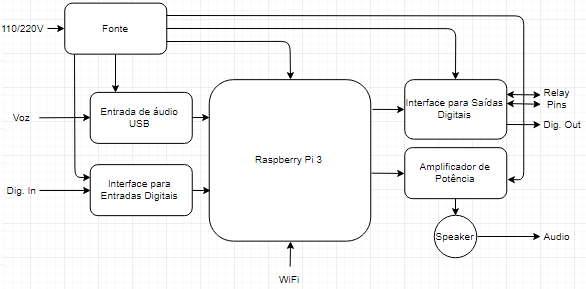
\includegraphics[scale=0.55]{projetoGeralHardware}
	\caption{Projeto Geral de Hardware}
	\label{fig-projetoGeralHardware}
\end{figure}


\subsection{Interface para Saídas e Entradas Digitais}

	\subsubsection{Saídas Digitais}
		A \textit{Raspberrry Pi3 Model B} possui 26 GPIOs \textit{(General Purpose Input/Output)} e as mesmas trabalham com nível lógico alto de 3V3 e nível lógico baixo de 0V. Isso de certa forma limita bastante as aplicações em que essas portas podem ser usadas, a maioria dos microcontroladores da família ATMega trabalham com nível lógico alto de 5V por exemplo, a indústria automotiva trabalha com nível lógico alto de 12V na maioria dos circuitos (exclui-se redes CAN). Em contrapartida é relativamente fácil modificar esse nível de tensão em questão visto que o mesmo se trata de um sinal digital. Uma solução relativamente simples consiste em utilizar as saídas digitais de 3V3 da \textit{RaspberrryPi} apenas para controlar circuitos que iram na prática acionar dispositivos externos em vez de acioná-los diretamente com a \textit{RaspberrryPi}. A Interface para saídas digitais pode ser dividida em dois circuitos replicáveis sendo o primeiro mostrado pela Figura \ref{fig-digitalOutput} a seguir.
		
		\begin{figure}[htbp]
			\centering
				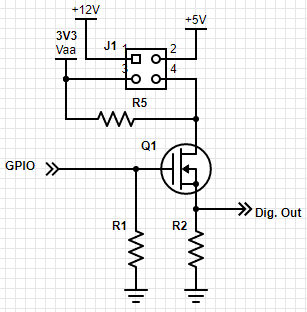
\includegraphics[scale=0.75]{digitalOutput}
			\caption{Circuito para Interface de Saídas Digitais}
			\label{fig-digitalOutput}
		\end{figure}

		Nesse circuito a GPIO polariza um \textit{MOSFET - (Metal–Oxide–Semiconductor Field-Effect Transistor} que pode ser conectado a diferentes fontes de tensão. Quando a GPIO envia um nível lógico alto o \textit{MOSFET} passa a conduzir a tensão escolhida (através do uso de um jumper) para a saída digital do dispositivo. Os resistores R1 e R2 são resistores de \textit{pull-down} (ambos de 10k$\Omega$ e servem para garantir que quando a GPIO não estiver enviando nível lógico alto o \textit{MOSFET} não estará polarizado e a saída do circuito será de nível lógico baixo (0V). Essa opção de poder escolher a tensão de saída é muito útil pois assim a \textit{RaspberrryPi} pode interfacear com diversos dispositivos, o resistor R5 é um resistor de \textit{pull-up} e é usado para garantir que quando nenhum jumper está conectado a tensão em nível lógico alto da saíad digital será de 3V3. 
	
	\subsubsection{Controle Relê}
	
	O circuito da interface de saídas digitais para controle do relê está apresentado na Figura \ref{fig-digitalOutputRelay} a seguir.
	
	\begin{figure}[htbp]
		\centering
			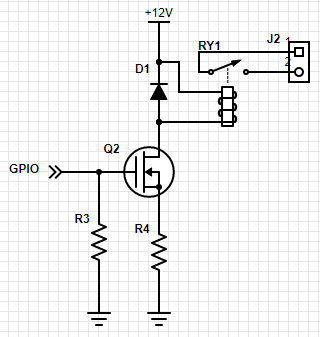
\includegraphics[scale=0.7]{digitalOutputRelay}
		\caption{Circuito para Interface de Controle de relê}
		\label{fig-digitalOutputRelay}
	\end{figure}
	
	Sobre o que involve o MOSFET esse circuito funciona de forma exatamente igual ao anterior, a diferença é que dessa vez em vez enviar um sinal digital esse circuito irá chavear um relê que pode controlar uma variedade maior de dispositivos, incluindo o uso de redes de corrente alternada, esmagadora maioria em redes residencias. O diodo serve para garantir que nenhuma corrente flua em sentido oposto ao ideal. Foi escolhido um MOSFET pois o mesmo não possui conexao física entre o terminal que está conectado na \textit{RaspberrryPi} e os demais e assim garante que apenas o resistor de \textit{pull-down} irá drenar corrente (uma corrente mínima poís o mesmo deverá ter valor altíssimo).

	\subsubsection{Interface para Entradas Digitais}

		Para que o dispositivo possa trabalhar com diferentes tensões na entrada digital será usado o circuito na Figura \ref{fig-digitalInput}.

		\begin{figure}[htbp]
			\centering
				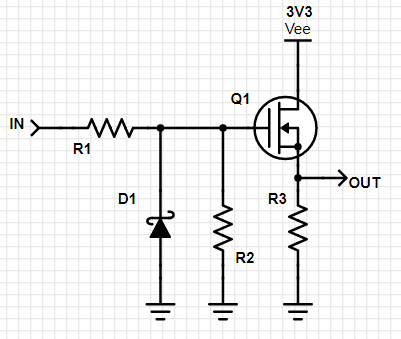
\includegraphics[scale=0.65]{digitalInput}
			\caption{Circuito para Interface de Entradas Digitais}
			\label{fig-digitalInput}
		\end{figure}
		
		O circuito converte uma tensão de qualquer valor maior que 3V3 em 3V3 em dois estágios. No primeiro estágio essa tensão é regulada para 3V3 usando o diodo zener (modelo 1N4728A) e depois polariza o mosfet que coloca 3V3 na saída. O resistor R1 serve para regular a corrente que passa pelo zener, a corrente máxima desse zener é de 276mA logo com o resistor R1 em 1k$\Omega$ o circuito pode trabalhar praticamente com qualquer tensão menor que 200V e maior que 3V3. O resistor R3 é um resistor de \textit{pull-down} e tem valor de 100k$\Omega$, é usado para garantir que a tensão de entrada no raspberry pi seja de 0V quando a tensão de entrada do circuito seja menor que 3V3. O Resistor R2 acabou não sendo montado pois foi julgado como desnecessário. 
		
	\subsubsection{Circuitos montados}
		Os três circuitos para interfaces digitais foram montados na mesma placa perfurada como mostra a Figura \ref{fig-digitalInterfaceCircuit}. Em todos os circuitos o mosfet escolhido foi o BS170.
		
		\begin{figure}[htbp]
			\centering
				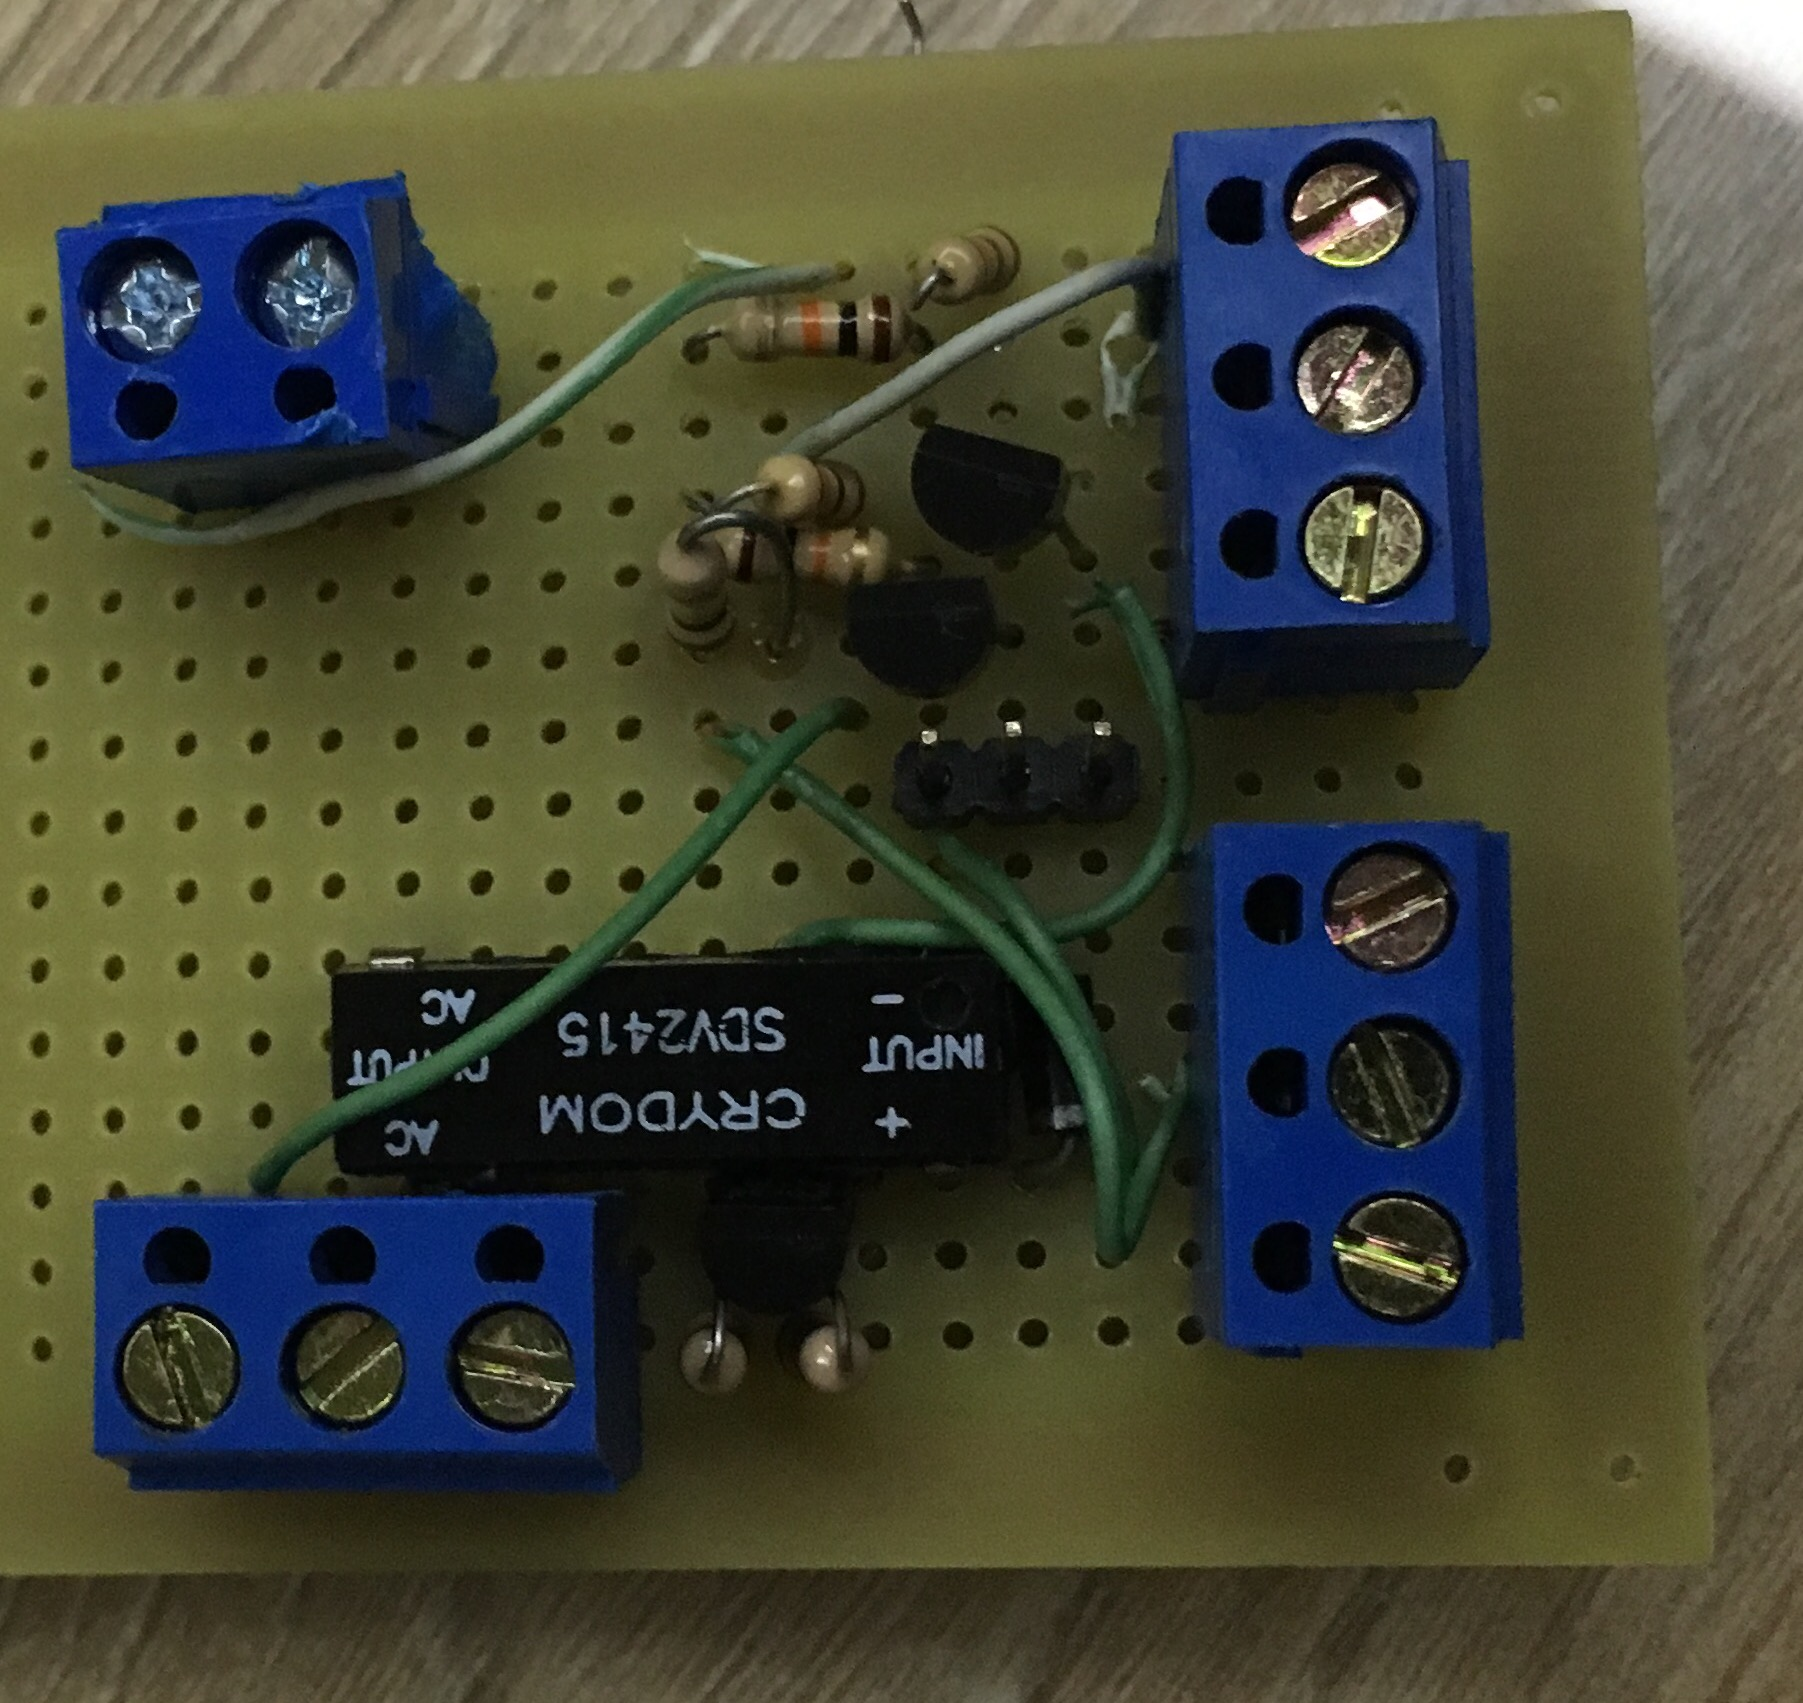
\includegraphics[scale=0.1]{digitalInterfaceCircuit}
			\caption{Circuito para Interfaces Digitais}
			\label{fig-digitalInterfaceCircuit}
		\end{figure}
		
		Os circuitos são perfeitamente escaláveis e por isso foi escolhido montar apenas um de cada para demonstrar o funcionamento.
	
\subsection{Amplificador de Potência}

	A saída de audio do \textit{RaspberrryPi} é apenas uma saída de sinal e para atender os requisitos do dispositivos proposto será necessário um amplificador de potência. O circuito da Figura \ref{fig-powerAmplifier} foi tirado da internet \cite{powerAmplifier} e é um amplificador com tensão de entrada de 12V e saída de 6W para um falante de 8Ohms (comum no mercado), esse circuito poderá ser modificado pois a potência do amplificador pode ser suficiente ou não para a aplicação.

	\begin{figure}[htbp]
		\centering
			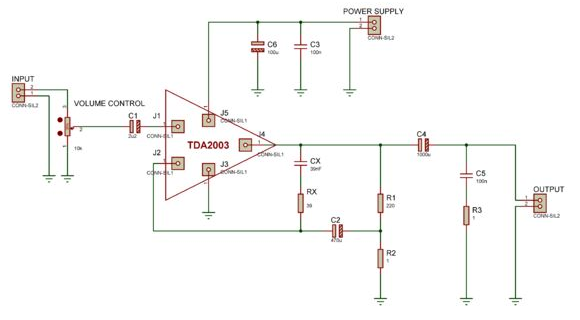
\includegraphics[scale=0.6]{powerAmplifier}
		\caption{Circuito para Amplificador de Potência}
		\label{fig-powerAmplifier}
	\end{figure}
	
	O circuito foi montado fielmente ao esquemático como mostra a Figura \ref{fig-powerAmplifierCircuit}.
	
	\begin{figure}[htbp]
		\centering
			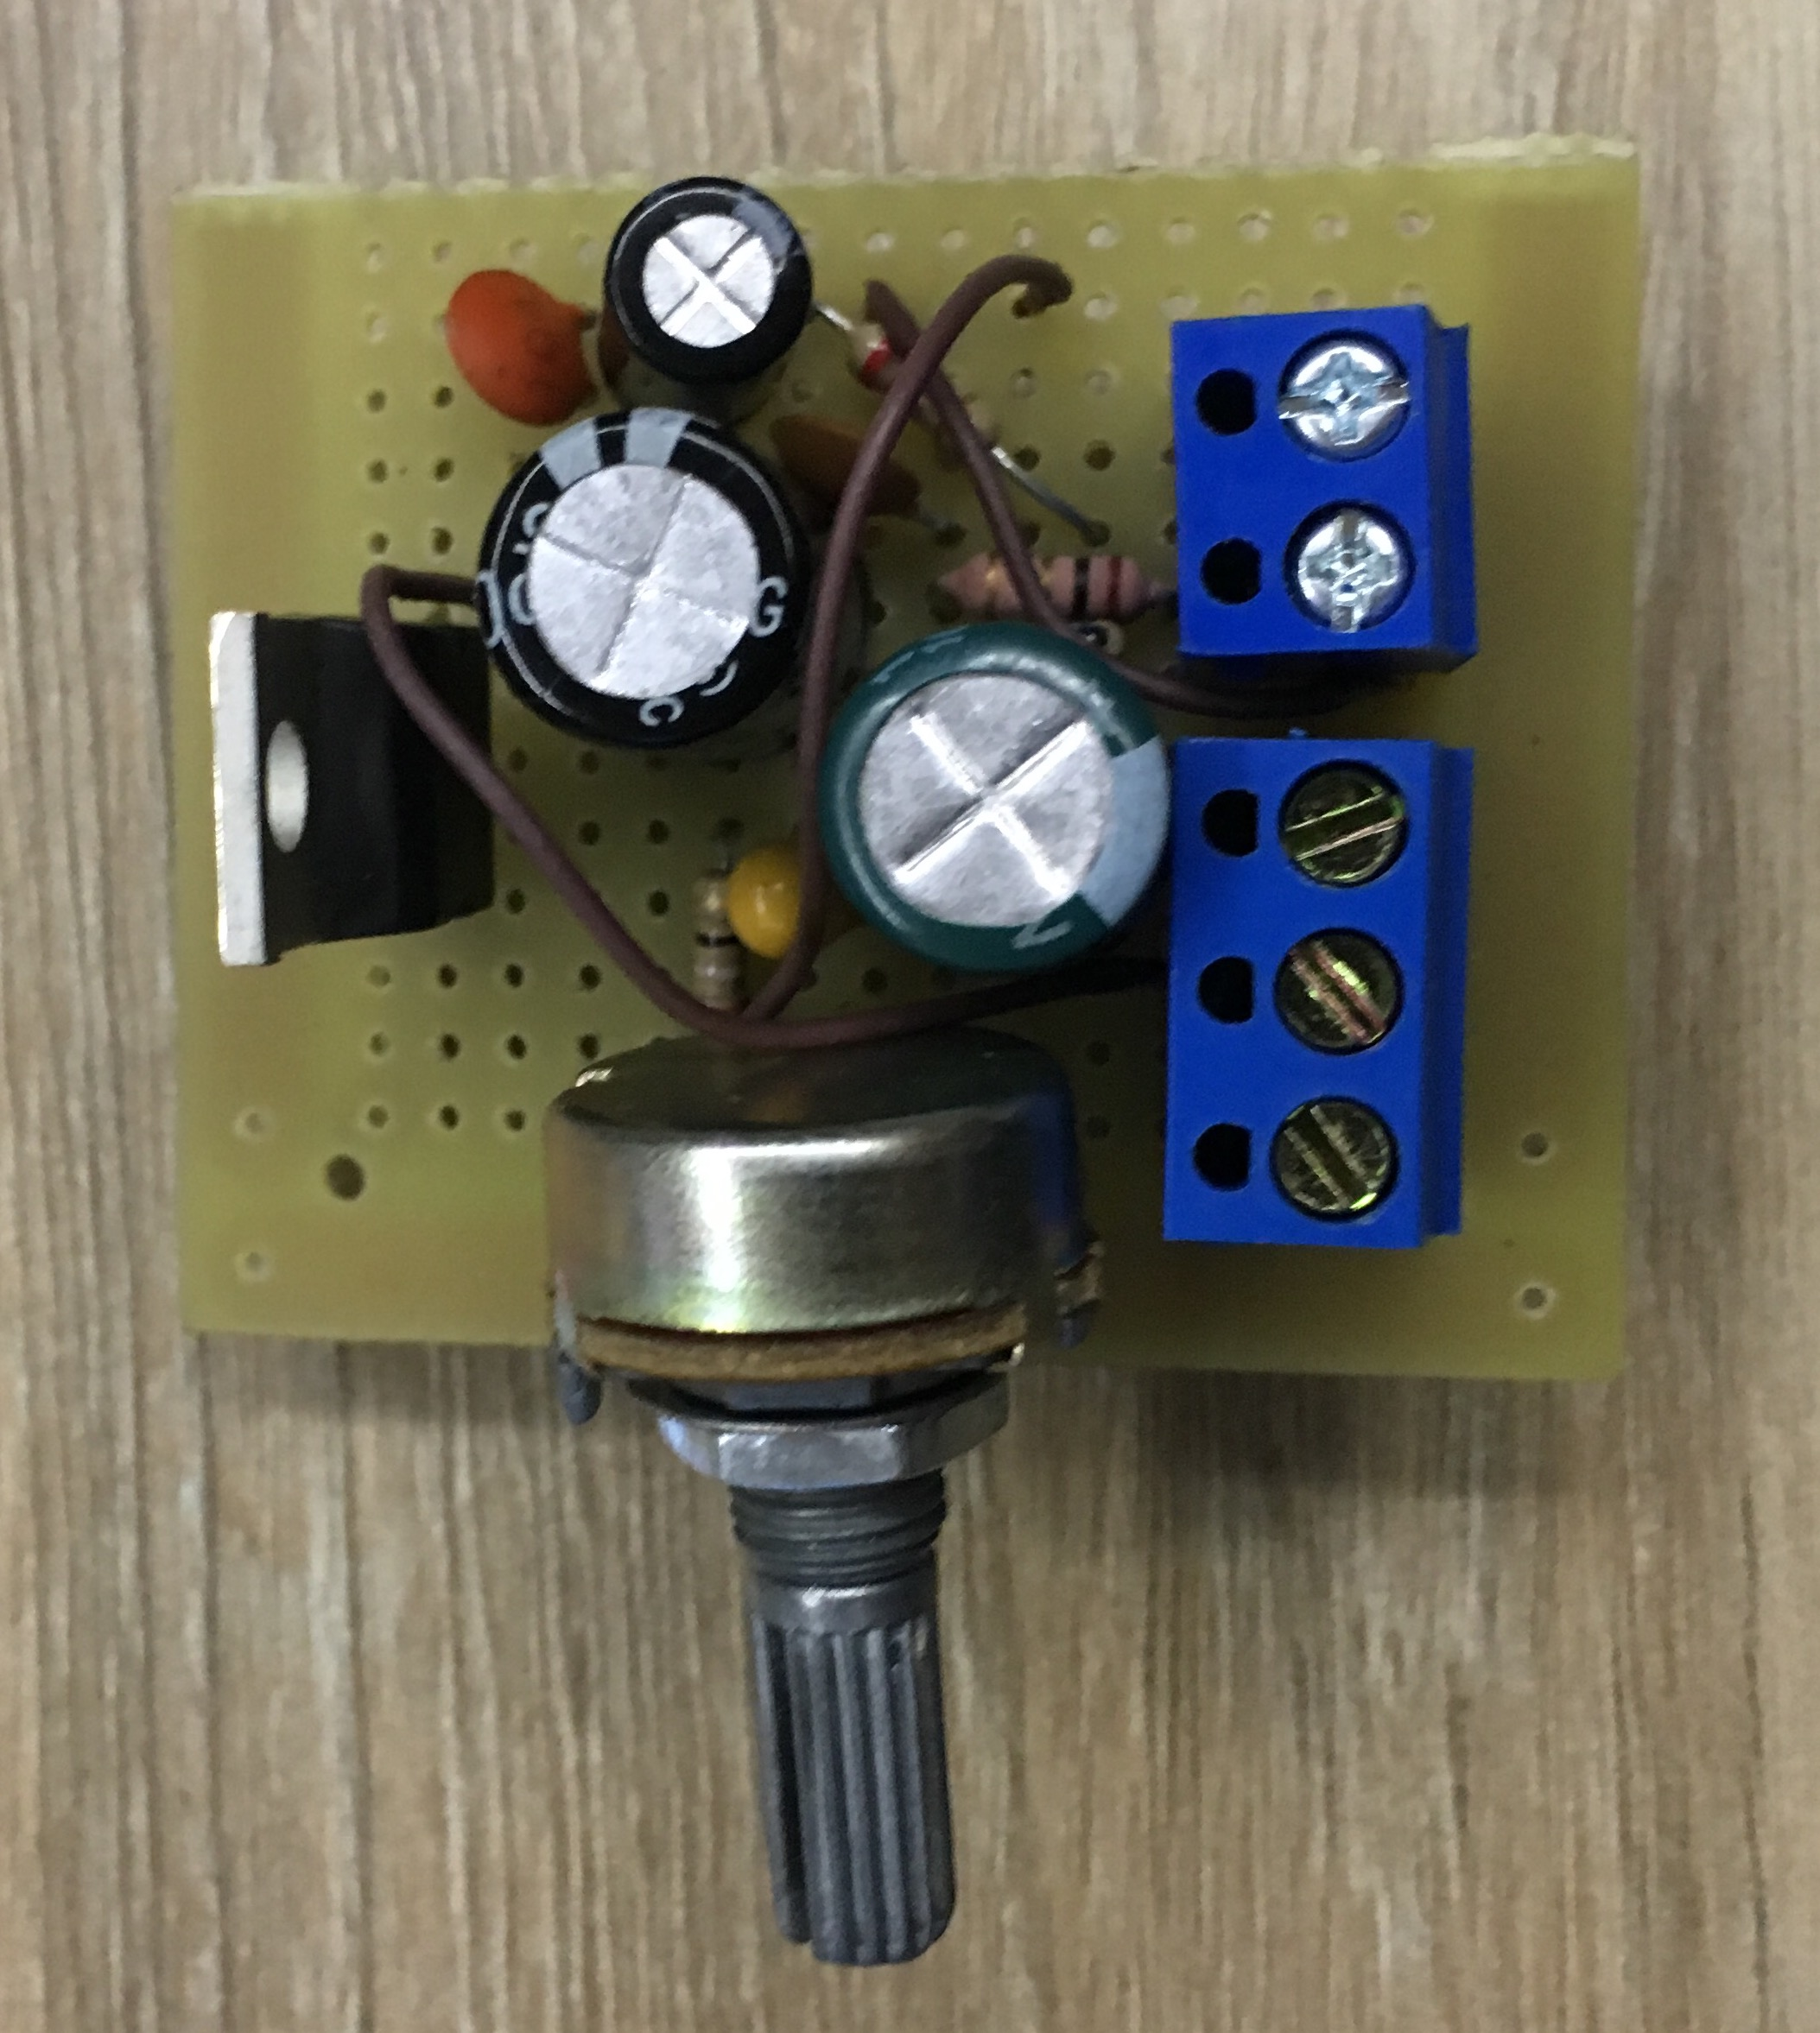
\includegraphics[scale=0.1]{powerAmplifierCircuit}
		\caption{Circuito Montado para o Amplificador de Potência}
		\label{fig-powerAmplifierCircuit}
	\end{figure}

\subsection{Fonte de Alimentação}

	Para o projeto será necessário ter fontes de tensão de três valores: 12V, 5V e 3V3. Como o foco desse projeto não é eletrônica de potência, será comprada uma fonte de 12V/DC e a tensão da mesma será convertida para os dois outros valores propostos: 5V e 3V3. Como a fonte de 5V é fundamental para o projeto será usado um regulador de tensão não-linear chaveado da \textit{Texas Instruments}, o componente escolhido é o LM2596 \cite{lm2596}. O mesmo pode fornecer até 3A na saída e possui eficiência de 80\%, o que elimina a necessidade de um dissipador grande de calor. Para a fonte de 3V3 será usado um regulador de tensão mais simples, o LM317 \cite{lm317}, apesar de ser um regulador mais simples a fonte de 3V3 será a menos demandada e por isso um regulador linear poderá ser usado. A Figura \ref{fig-powerSouce} mostra o projeto das fontes de alimentação.
	
	\begin{figure}[htbp]
		\centering
			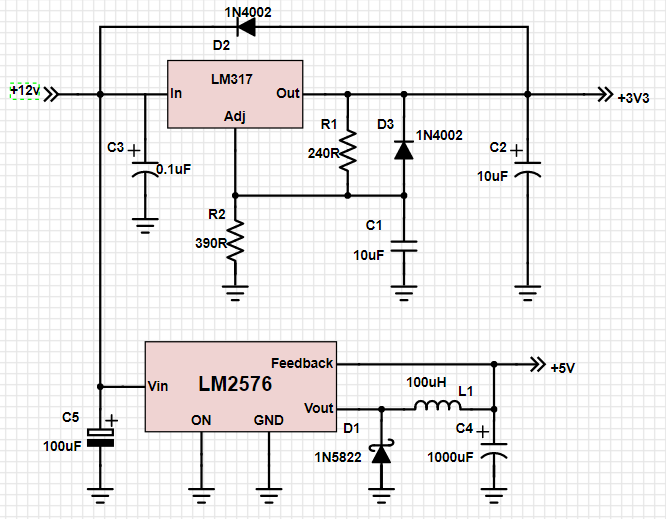
\includegraphics[scale=0.5]{powerSource}
		\caption{Fonte de Alimentação}
		\label{fig-powerSouce}
	\end{figure}
	
	A escolha dos componentes adjacentes aos reguladores foi feita de acordo com as recomendações dos datasheets.  
	
	O circuito foi montado fielmente ao esquemático como mostra a Figura \ref{fig-powerSourceCircuit}.
	
	\begin{figure}[htbp]
		\centering
			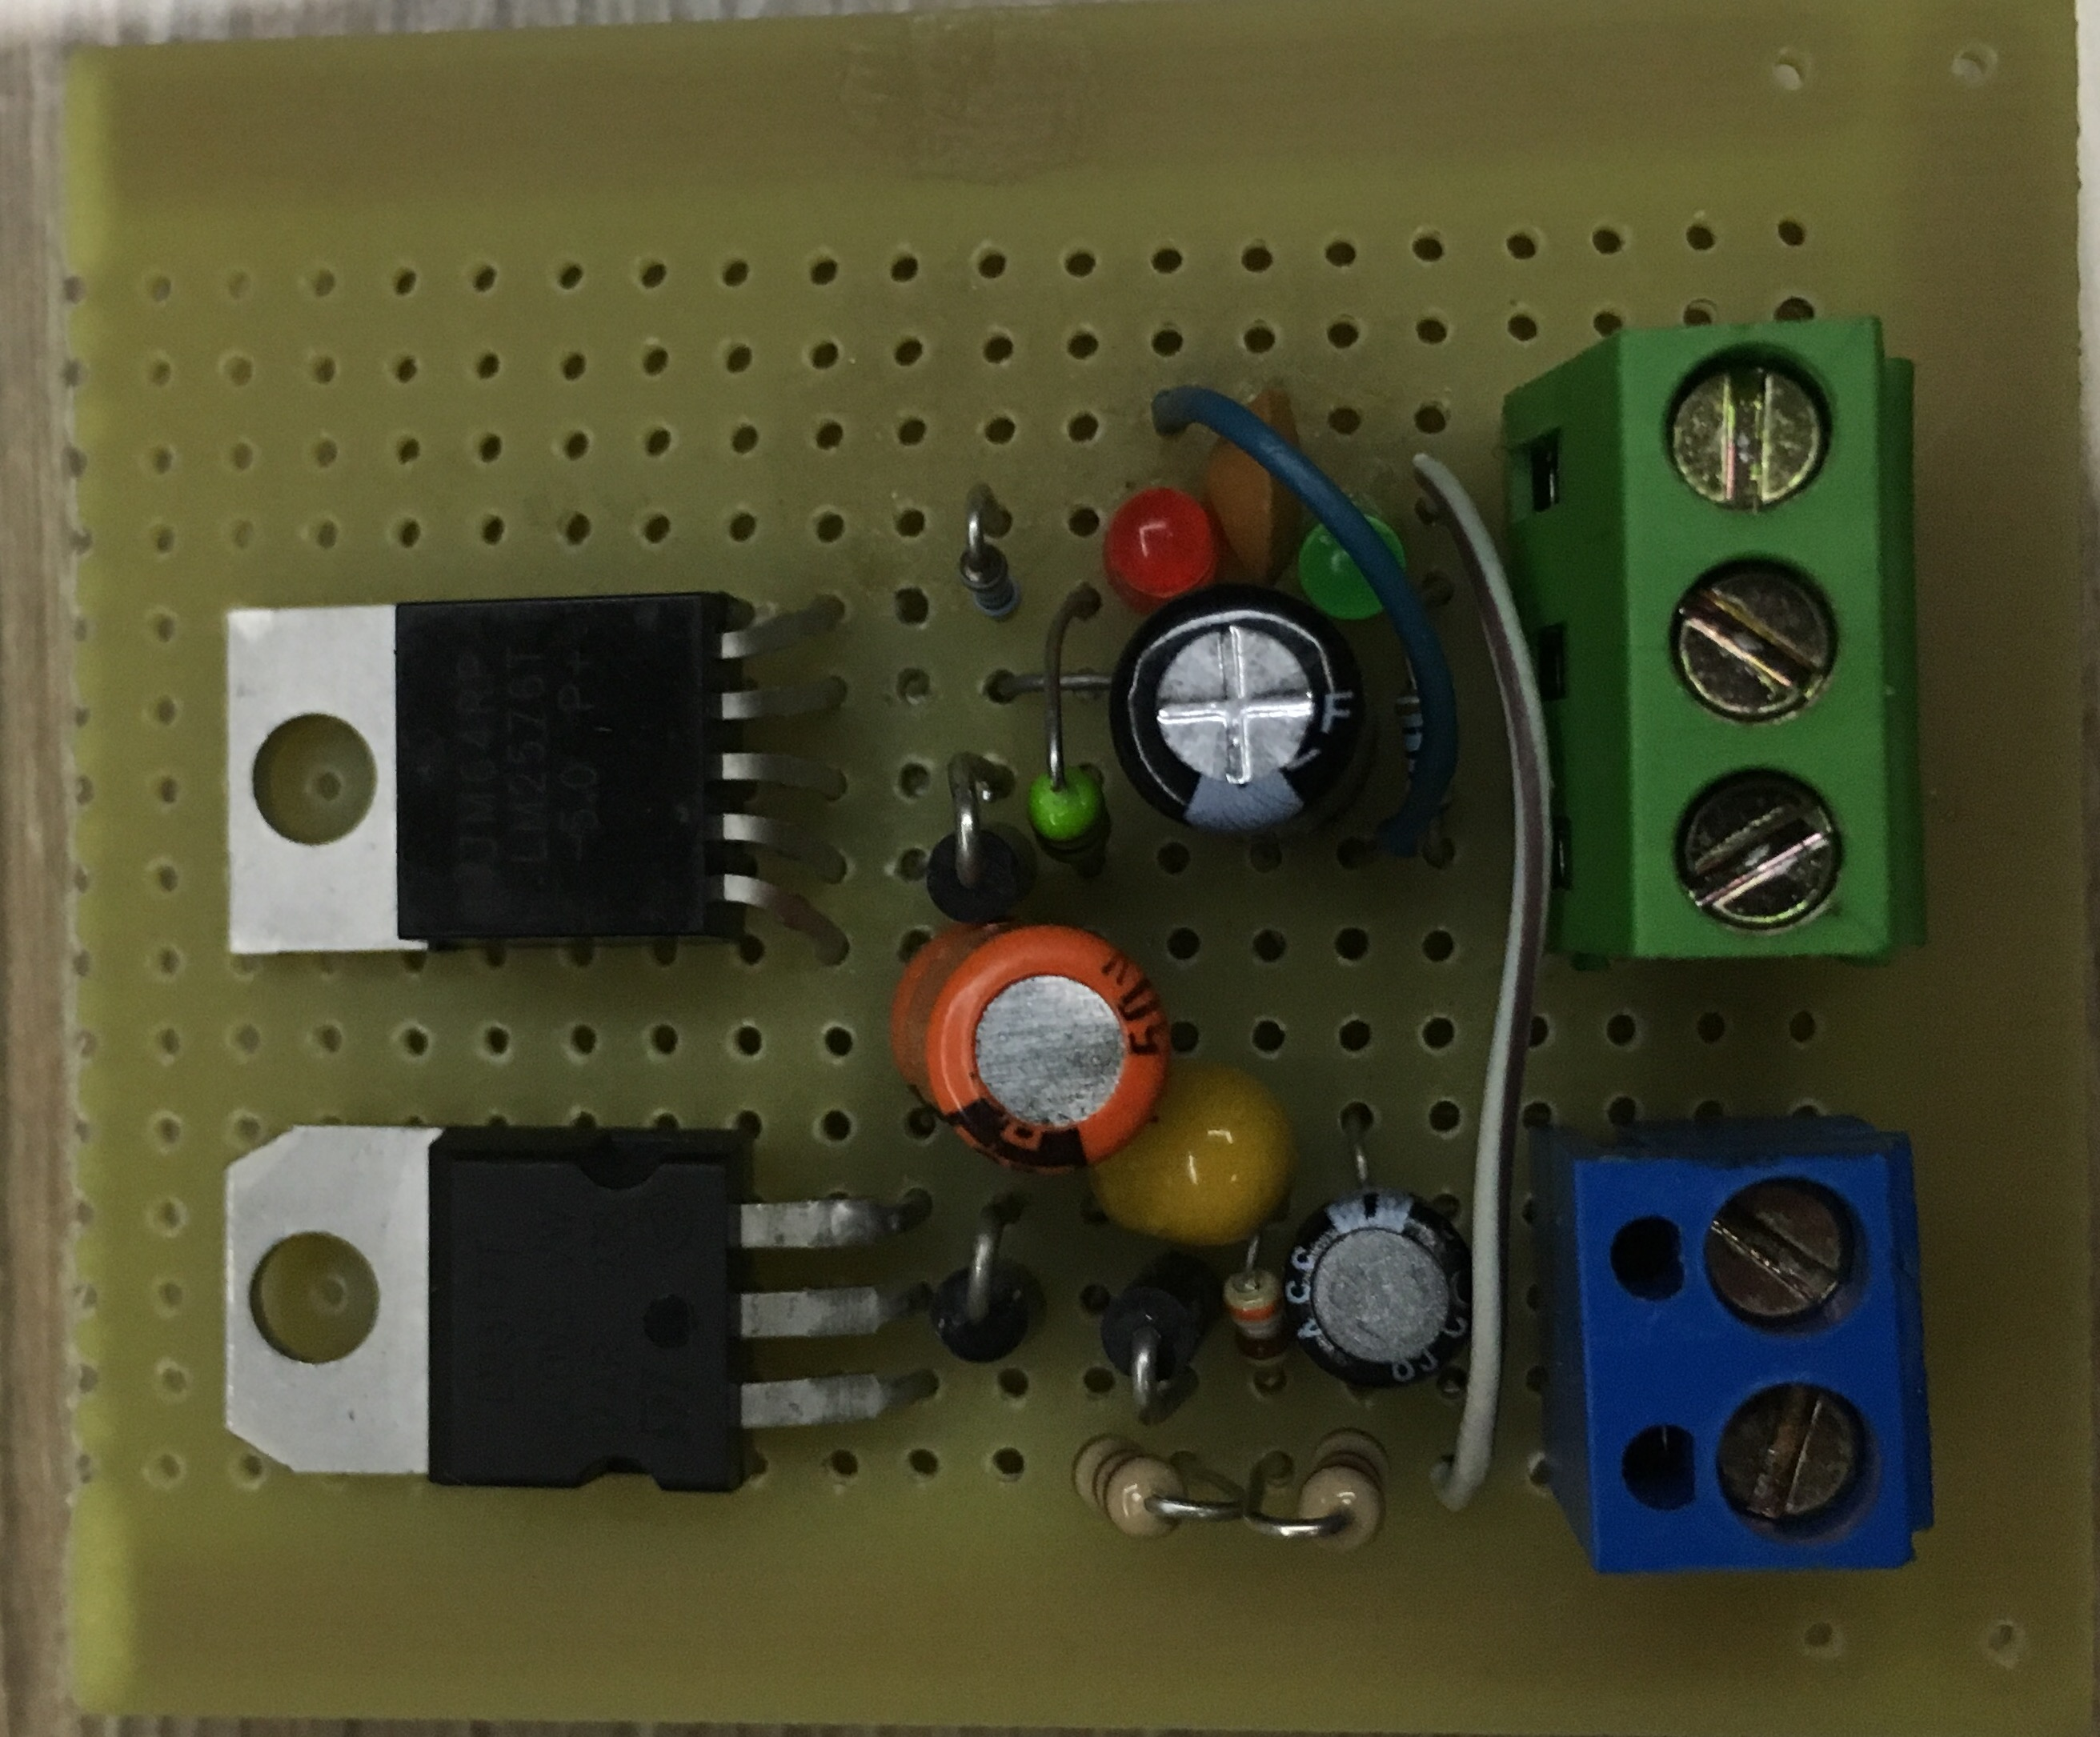
\includegraphics[scale=0.1]{powerSourceCircuit}
		\caption{Circuito Montado para Fonte de Alimentação}
		\label{fig-powerSourceCircuit}
	\end{figure}
